%!TEX TS-program = xelatex
\documentclass[12pt, a4paper, oneside]{article}

\usepackage{amsmath,amsfonts,amssymb,amsthm,mathtools}  % пакеты для математики

\usepackage[utf8]{inputenc} % задание utf8 кодировки исходного tex файла
\usepackage[british,russian]{babel} % выбор языка для документа

\usepackage{fontspec}         % пакет для подгрузки шрифтов
\setmainfont{Helvetica}   % задаёт основной шрифт документа

% why do we need \newfontfamily:
% http://tex.stackexchange.com/questions/91507/
\newfontfamily{\cyrillicfonttt}{Helvetica}
\newfontfamily{\cyrillicfont}{Helvetica}
\newfontfamily{\cyrillicfontsf}{Helvetica}

\usepackage{unicode-math}     % пакет для установки математического шрифта
\setmathfont{Neo Euler}      % шрифт для математики
% \setmathfont[math-style=ISO]{Asana Math}
% Можно делать смену начертания с помощью разных стилей

% Конкретный символ из конкретного шрифта
% \setmathfont[range=\int]{Neo Euler}

%%%%%%%%%% Работа с картинками %%%%%%%%%
\usepackage{graphicx}                  % Для вставки рисунков
\usepackage{graphics}
\graphicspath{{images/}{pictures/}}    % можно указать папки с картинками
\usepackage{wrapfig}                   % Обтекание рисунков и таблиц текстом

%%%%%%%%%%%%%%%%%%%%%%%% Графики и рисование %%%%%%%%%%%%%%%%%%%%%%%%%%%%%%%%%
\usepackage{tikz, pgfplots}  % язык для рисования графики из latex'a

%%%%%%%%%% Гиперссылки %%%%%%%%%%
\usepackage{xcolor}              % разные цвета

\usepackage{hyperref}
\hypersetup{
	unicode=true,           % позволяет использовать юникодные символы
	colorlinks=true,       	% true - цветные ссылки, false - ссылки в рамках
	urlcolor=blue,          % цвет ссылки на url
	linkcolor=red,          % внутренние ссылки
	citecolor=green,        % на библиографию
	pdfnewwindow=true,      % при щелчке в pdf на ссылку откроется новый pdf
	breaklinks              % если ссылка не умещается в одну строку, разбивать ли ее на две части?
}


\usepackage{todonotes} % для вставки в документ заметок о том, что осталось сделать
% \todo{Здесь надо коэффициенты исправить}
% \missingfigure{Здесь будет Последний день Помпеи}
% \listoftodos --- печатает все поставленные \todo'шки

\usepackage[paper=a4paper, top=20mm, bottom=15mm,left=20mm,right=15mm]{geometry}
\usepackage{indentfirst}       % установка отступа в первом абзаце главы

\usepackage{setspace}
\setstretch{1.15}  % Межстрочный интервал
\setlength{\parskip}{4mm}   % Расстояние между абзацами
% Разные длины в латехе https://en.wikibooks.org/wiki/LaTeX/Lengths


\usepackage{xcolor} % Enabling mixing colors and color's call by 'svgnames'

\definecolor{MyColor1}{rgb}{0.2,0.4,0.6} %mix personal color
\newcommand{\textb}{\color{Black} \usefont{OT1}{lmss}{m}{n}}
\newcommand{\blue}{\color{MyColor1} \usefont{OT1}{lmss}{m}{n}}
\newcommand{\blueb}{\color{MyColor1} \usefont{OT1}{lmss}{b}{n}}
\newcommand{\red}{\color{LightCoral} \usefont{OT1}{lmss}{m}{n}}
\newcommand{\green}{\color{Turquoise} \usefont{OT1}{lmss}{m}{n}}

\usepackage{titlesec}
\usepackage{sectsty}
%%%%%%%%%%%%%%%%%%%%%%%%
%set section/subsections HEADINGS font and color
\sectionfont{\color{MyColor1}}  % sets colour of sections
\subsectionfont{\color{MyColor1}}  % sets colour of sections

%set section enumerator to arabic number (see footnotes markings alternatives)
\renewcommand\thesection{\arabic{section}.} %define sections numbering
\renewcommand\thesubsection{\thesection\arabic{subsection}} %subsec.num.

%define new section style
\newcommand{\mysection}{
	\titleformat{\section} [runin] {\usefont{OT1}{lmss}{b}{n}\color{MyColor1}} 
	{\thesection} {3pt} {} } 


%	CAPTIONS
\usepackage{caption}
\usepackage{subcaption}
%%%%%%%%%%%%%%%%%%%%%%%%
\captionsetup[figure]{labelfont={color=Turquoise}}

\pagestyle{empty}

\begin{document}

\section*{Задание 2  (20 + 15 баллов)}

Не забывай, где находится  \href{https://fulyankin.github.io/LaTeX/}{страничку курса} с кучей шпаргалок!

\textbf{Символический дедлайн:  28 февраля.} В этой домашке несколько простых заданий, позволяющих вам ещё больше освоиться в \LaTeX{.}  Вы можете сделать то количество заданий, которое захотите. (Это правда, вы очень большой молодец, когда не ленитесь. Более того, вы ещё и очень красивы.) 

Когда вы сделали ровно столько задач, сколько хотите, то вам нужно:

\begin{enumerate}
\item Проверить точно ли файл без ошибок компилируется на вашем компьютере.
\item Убедиться, что каждое упражнение оформлено в отдельном файле.
\item Положить все свои наработки в отдельную папочку.
\item Удалить все промежуточные файлы. В папке должны остаться только .tex, .pdf, картинки. Если вы использовали нестандартный шрифт, положите файл с ним в папочку.
\item Положить папку на	свой	Dropbox, Github,	yandex-disk	или другой	репозиторий.
\item Заполнить	\href{https://docs.google.com/forms/d/e/1FAIpQLSe11kxKVfv07iCL1E9yNX7ll9swKImiVwRr1H70lslGzInRSg/viewform}{уютную гугл-форму.} Ради всего святого называйте свои папки в формате: номер дз Фамилия Имя. Например: 2 Петров Пётр.
\item Не стесняйтесь абсолютно в любое время дня и ночи просить о помощи, если она вам действительно необходима! Также не забывайте про то, что любое творчество поощряется. 
\end{enumerate}

\subsection*{[5]  Упражнение 1 }

\begin{itemize}
	\item[$(1)$]  Подключите словари для проверки орфографии. Введите какое-нибудь слово с грамматической ошибкой и его же без ошибки. Сделайте скриншот и приложите его к домашке. 
	\item [$(2)$]  Поставьте \href{https://www.ctan.org/pkg/excel2latex}{надстройку на excel} для создания таблиц и сделайте какую угодно таблицу. 
	\item[$(2)$]  Установите на свой компьютер \href{https://www.geogebra.org/download}{Geogebra}, нарисуйте какой-нибудь рисунок экспортируете его в \LaTeX также как мы делали это на паре. 
\end{itemize}


\subsection*{[5]  Упражнение 2 (Право на ошибку)}

\todo[inline]{Поставить ссылку на необходимые материалы}

Каждый человек имеет право на ошибку. Иногда даже на много ошибок. При условии, если человеку помогут его ошибки исправить. Саша совсем недавно начал изучать LaTeX. Он допустил довольно большое количество ошибок...

Вот файл, который Саша набирал. Исправьте все ошибки Саши и заставьте файл работать! Больше никогда такие ошибки не допускайте. Если исправлены все ошибки и файл собирается, то вы получаете 4 балла. Если исправлены все Warning, вы получаете 5 баллов. Если вы осознаёте что вы только что прочитали, то вы получаете плюс к карме.


\subsection*{[10]  Упражнение 3 (Где деньги, Лебовски?)}

Найдите в интернете какой-нибудь крутой шрифт.  Например, я точно знаю что есть шрифт в стиле Гарри Поттера или шрифт в стиле Игры Престолов. Напишите короткое послание в стилистике этого шрифта. Наример, предупреждение о вторжении, тайное послание и т.п. 

Если лень выдумывать, то просто напишите мне или одному из проверяющих с помощью шрифта вымогателей угрозу.  Не забудьте подписать работу...   Times New Roman, Arial и тп интересными шрифтами не считаются!

\begin{center}
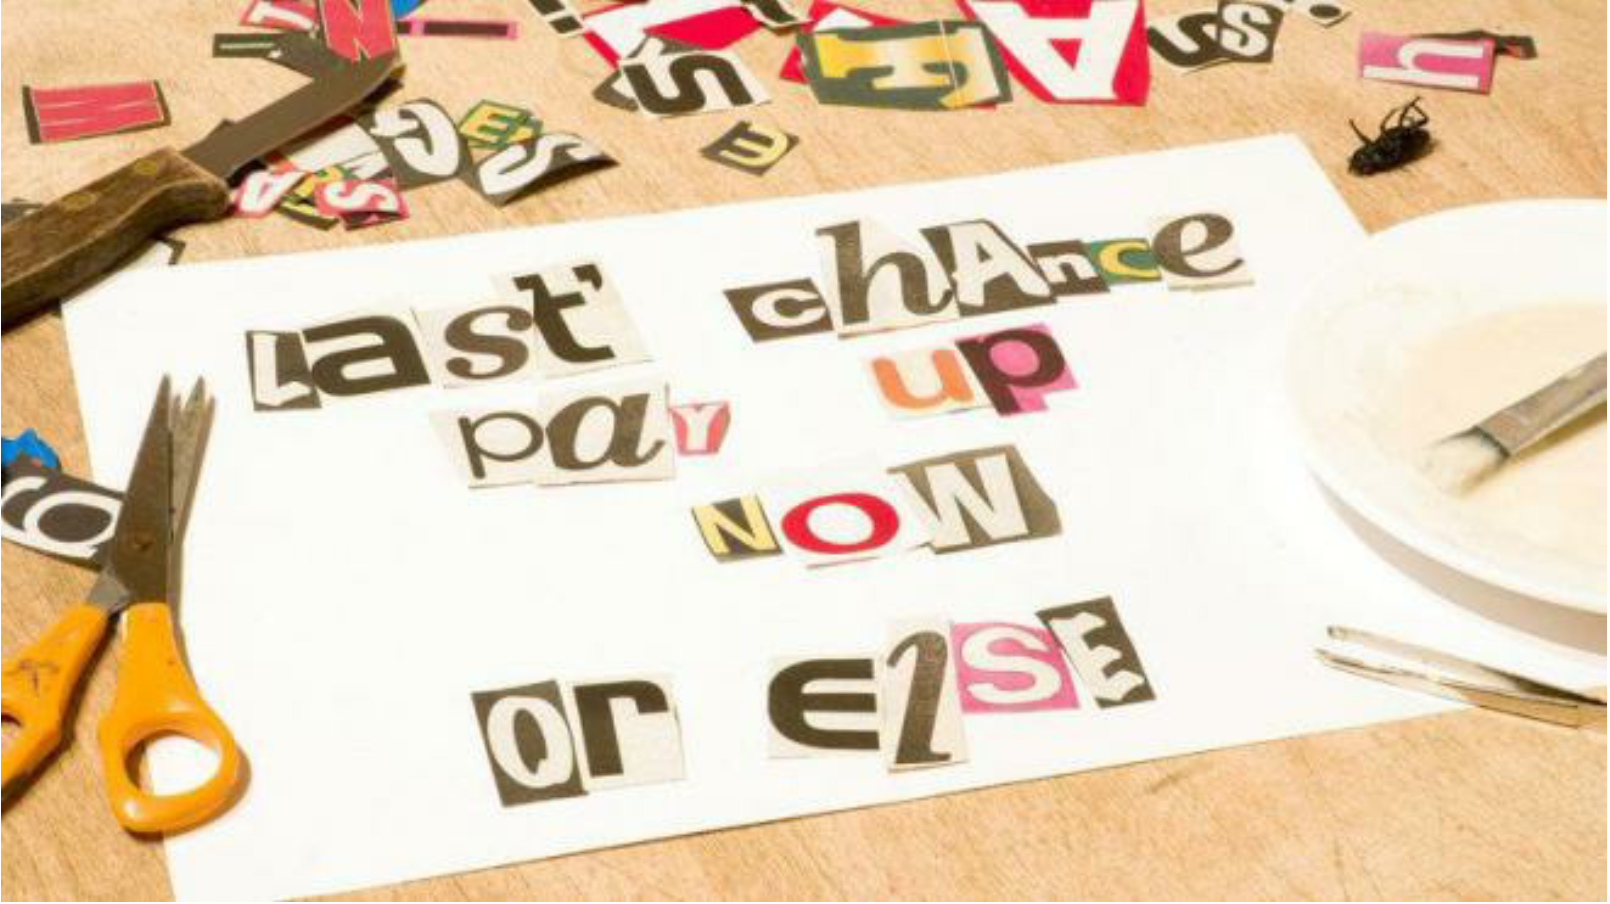
\includegraphics[scale=0.2]{letters.png}
\end{center} 


\subsection*{[15]  Упражнение 4 (На все ваши ответы будут заданы вопросы)}

\textbf{Это упражнение  является дополнительным.}  В легендах всех основных культур присутствует персонаж, который выполняет желания. У арабов джин, у ирландцев леприкон, у китайцев дракон и обезьяна, у русских золотая рыбка, щука, цветик-семицветик, старик Хоттабыч, двое из ларца, дед Мороз (и это ещё не полный список), а у американцев он. О. Ж. Грант.

Иногда особым счастливчикам доводится встретить О.Ж. Гранта в окрестностях Трассы 60 и поработать на него. В этих особых ситуациях им приходится подписать контракт.

Когда вы гуляли по улицам одного маленького американского городка, на вашем пути возник таинственный незнакомец. Вы сразу догадались кто перед вами и согласились выполнить его задание. Однако у мистера Гранта кончились экземпляры контрактов. К счастью, у вас под рукой есть компьютер. Напишите в \LaTeX{} экземпляр контракта для мистера Гранта. Он должен выглядеть примерно вот так:

\begin{center}
	
\includegraphics[scale=0.4]{Hg91uSv1cik.jpg}
	
\includegraphics[scale=0.4]{t_XxgIqEmBE.jpg}
\end{center} 

Полулеприкон любит творческих людей. Если вы именно такой человек, то при выполнении вашего желания он вас не обманет. И главное: не забывайте, если человек настроен серьёзно, то он не пожалеет для заключения договора капли крови.

\begin{itemize}
\item[$(5)$]   Вами был составлен контракт для О.Ж. Гранта, который как минимум включает в себя:

\begin{enumerate}
\item  Место для подписи.
\item  Место для крови.
\item  Готический заголовок.
\item  Бумага, на которой оформлен контракт немного состарена.
\item  При оформлении контракта оставьте в преамбуле только те пакеты, которые реально используются в документе.
\end{enumerate}

\item[$(10)$] Вы распечатали контракт, поставили подпись, скрепили его кровью и сдали лектору. Для наших целей наличие крови или вещества, которое имитирует её обязательно!
\end{itemize}

\textbf{Подсказки:}  Помните о Tikz. В нём можно нарисовать абсолютно любой элемент декора для вашего документа. Обратите внимание, что разбрызганная кровь чем-то напоминает разлитые чернила.

\end{document}
